% C.13 SAS: AB=AD, ∠BAC=∠DAC, AC 公共
\documentclass[tikz,border=4pt]{standalone}
\usepackage{ctex}
\usepackage{amsmath}
\usetikzlibrary{calc, arrows.meta,decorations.markings}
\begin{document}
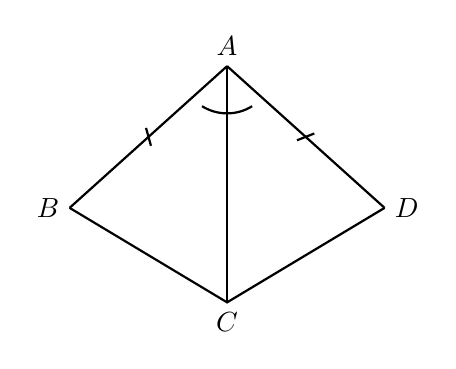
\begin{tikzpicture}[scale=1.0, thick,
  tickone/.style={postaction={decorate, decoration={markings,
    mark=at position 0.5 with {\draw (-1.5pt,-3pt) -- (1.5pt,3pt);}}}}]
  \coordinate (A) at (0,2.4);
  \coordinate (C) at (0,-0.6);
  \coordinate (B) at (-2,0.6);
  \coordinate (D) at (2,0.6);
  \draw[tickone] (A) -- (B);
  \draw[tickone] (A) -- (D);
  \draw (A) -- (C);
  \draw (B) -- (C) -- (D);
  \node[above] at (A) {$A$};
  \node[left] at (B) {$B$};
  \node[right] at (D) {$D$};
  \node[below] at (C) {$C$};
  % 双弧表示∠BAC=∠DAC
  \draw (0,1.8) arc (-90:-90+32:0.6);
  \draw (0,1.8) arc (-90:-90-32:0.6);
\end{tikzpicture}
\end{document}
